% =====================================================================
% main.tex --- Territorial Belief on Theory-of-Space
% NeurIPS-style course-project proposal / open-defense draft.
%
% Recommended Overleaf setup (one-click):
%   1. New Project -> Templates -> NeurIPS 2024 (or 2025 if available)
%   2. Replace main.tex with this file.
%   3. Drop the figures/ folder (already exported as .pdf and .png) at
%      the project root.
%   4. Compile with pdfLaTeX. (XeLaTeX also works.)
%
% If the official NeurIPS sty is not available, the document still
% compiles under article+10pt with mild visual differences.
% =====================================================================

\documentclass{article}

% --- Try the official NeurIPS style; fall back to plain article. -----
\IfFileExists{neurips_2025.sty}{%
  \usepackage[final]{neurips_2025}
}{%
  \IfFileExists{neurips_2024.sty}{%
    \usepackage[final]{neurips_2024}
  }{%
    % Fallback: tighten margins so the layout looks NeurIPS-ish.
    \usepackage[margin=1in]{geometry}
  }
}

% --- Encoding / font / language ---------------------------------------
\usepackage[utf8]{inputenc}
\usepackage[T1]{fontenc}
\usepackage{lmodern}
\usepackage{microtype}

% --- Math / theorem ---------------------------------------------------
\usepackage{amsmath,amssymb,amsthm}
\usepackage{mathtools}
\usepackage{bm}
\newtheorem{proposition}{Proposition}
\newtheorem{definition}{Definition}

% --- Figures / floats / tables ---------------------------------------
\usepackage{graphicx}
\graphicspath{{figures/}{../figures/}}
\usepackage{booktabs}
\usepackage{multirow}
\usepackage{caption}
\usepackage{subcaption}

% --- Algorithms (used in §3.1) ---------------------------------------
\usepackage{algorithm}
\usepackage{algpseudocode}

% --- Hyperref + cleveref MUST be loaded LAST -------------------------
\usepackage[colorlinks=true,linkcolor=blue!50!black,citecolor=blue!50!black,urlcolor=blue!50!black]{hyperref}
\usepackage{cleveref}

% --- Custom shorthands ------------------------------------------------
\newcommand{\tos}{\textsc{Theory-of-Space}\xspace}
\newcommand{\tb}{\textsc{TerritorialBelief}\xspace}
\newcommand{\stab}{\mathrm{Stab}}
\newcommand{\inertia}{\mathrm{Inertia}}
\newcommand{\R}{\mathbb{R}}
\newcommand{\N}{\mathbb{N}}
\newcommand{\E}{\mathbb{E}}
\usepackage{xspace}

% --- Title / authors --------------------------------------------------
\title{Territorial Belief for Active Spatial Exploration:\\
A Diagnostic Extension of \tos}

\author{%
  Cora \\
  Brain \& Machine Intelligence (08), Spring 2026 \\
  \texttt{f\_raike@mail.com} \\
}

\begin{document}
\maketitle

% =====================================================================
\begin{abstract}
The recent ICLR-2026 \tos benchmark reframes spatial intelligence as the
ability to \emph{actively} construct, revise, and exploit an internal
spatial belief, and reveals two characteristic failures of large
multimodal foundation models: (i) \emph{belief drift}---previously correct
predictions get silently corrupted in later turns---and (ii) \emph{belief
inertia}---when objects move, the model fails to overwrite obsolete
priors. We argue that both failures share a common root: foundation
models maintain a flat coordinate-level belief with no structural unit at
which to anchor stability or to localise revision. Drawing on
hippocampal place/grid-cell biology and animal territoriality, we
introduce \tb, a representation that organises objects under
room-level latent units, accumulates familiarity, and gates updates via
a confidence buffer. We formalise the representation, plug it as a
diagnostic baseline into the official \tos benchmark, and show in
preliminary smoke-test runs that \tb improves Stability and orientation
Correctness over a free-form LLM cognitive map, at a measurable
sub-cell-precision cost on positional Perception. Full-scale Qwen-VL-7B
runs on 25 procedurally generated 3-room scenes (text \& vision worlds)
are scheduled for the next two days; the open-defence is built around
the methodology, the formal model, and these preliminary numbers.
\end{abstract}
% =====================================================================

\section{Introduction}\label{sec:intro}

Foundation models that pass disembodied spatial-reasoning benchmarks
(\textit{e.g.\ } SpartQA \citep{mirzaee2021spartqa}, SpatialVLM
\citep{chen2024spatialvlm}, MMSI-Bench \citep{yang2025mmsi}) struggle
once the agent must \emph{actively} acquire information under partial
observability. \tos \citep{zhang2026theoryofspace} formalises this gap by
asking foundation-model agents to (i) decide what to observe next,
(ii) externalise their cognitive map at every turn, and (iii) revise
that map after a covert false-belief perturbation. Across GPT-5.2,
Gemini-3-Pro, Claude-4.5-Sonnet and three open-source vision-language
models, \tos identifies two consistent failure modes:

\begin{itemize}
\item \textbf{Belief drift} (\tos\,\S5.1): a previously correct
prediction has only $\sim$57--67\% probability of remaining correct in
the next turn (vision-world Stability scores).

\item \textbf{Belief inertia} (\tos\,\S5.3): after objects are silently
relocated, vision agents persist with the obsolete coordinates
\emph{despite directly observing} the new layout (positional inertia
35--69\%, orientational inertia 51--69\%).
\end{itemize}

\paragraph{Hypothesis.}
Both failures share a common architectural root: foundation models
maintain a \emph{flat} belief over individual object coordinates, with
no intermediate structural unit at which (a) to anchor temporal
stability or (b) to localise revision when the world changes. The
mammalian brain does not store space this way: place cells
\citep{okeefe1971} and grid cells \citep{hafting2005} provide a
\emph{region-level} code, and animal territoriality
\citep{burt1943,powell2012homerange} organises familiarity, ownership,
and recovery at the level of the \emph{home range}. Recent neural-AI
replications \citep{banino2018grid} show region-level codes emerge
spontaneously even in artificial agents.

\paragraph{Contribution.}
We introduce \tb, a structurally region-level belief representation,
and plug it as a diagnostic baseline into the \tos benchmark. \tb
organises observed objects under room-level latent units, accumulates a
visit-and-recency familiarity signal, and gates per-object updates by a
confidence buffer that requires \emph{two} contradictory observations
before overwriting a stored fact. We:

\begin{enumerate}
\item formalise \tb as an extension of the \tos belief
$\hat B_t \in \mathcal{J}$ (Section~\ref{sec:method});

\item analytically derive the consequence on Stability and
Belief~Inertia (Section~\ref{sec:method}, full proofs in
Appendix~\ref{app:math});

\item implement a Python post-hoc replay tool that ingests the
\tos exploration log and emits a parallel \tb cognitive map per turn,
without retraining or re-rolling the underlying LLM
(Section~\ref{sec:setup});

\item report preliminary smoke-test numbers and the planned full
Qwen-VL-7B runs (Section~\ref{sec:results}--\ref{sec:plan}).
\end{enumerate}

The framing is explicitly diagnostic rather than performance-chasing:
the goal is to expose \emph{which} \tos failure modes are tied to the
flatness of LLM cognitive maps and which are not, by substituting a
structurally different cognitive map into the same probing pipeline.


\section{Related Work}\label{sec:related}

% Condensed from lit_review_condensed.md; ~3/4 column.
\paragraph{From passive to active spatial reasoning.}
Static-scene benchmarks \citep{weston2015babi,shi2022stepgame,
mirzaee2021spartqa,chen2024spatialvlm,ma20243dsr,yang2025mmsi} evaluate
disembodied spatial reasoning. A second wave introduced
\emph{cognitive-map prediction} as an auxiliary objective:
VSI-Bench \citep{yang2025vsi} and MindCube \citep{yin2025mindcube}
showed that explicit map prediction improves video and multi-view QA.
\tos \citep{zhang2026theoryofspace} departs from both lines: the agent
itself decides what to observe next, externalises its cognitive map at
every step (probing), and is tested under a \emph{false-belief}
perturbation borrowed from developmental psychology
\citep{wimmer1983false}. \tos provides the only published probing
benchmark that simultaneously evaluates Stability, Self-tracking,
Local$\leftrightarrow$Global consistency, and Belief Inertia under a
single representation.

\paragraph{Cognitive maps in neuroscience and bio-inspired AI.}
Place cells \citep{okeefe1971}, grid cells \citep{hafting2005}, and
their hierarchical structure \citep{stensola2012} encode space at the
region level rather than as a flat coordinate list. Banino~et~al.\
\citep{banino2018grid} showed that grid-like codes \emph{spontaneously
emerge} in deep RL agents; MoHA (Motivational Cognitive Maps,
\citet{mohacog2025}) modulates the spatial map by motivational
signals; RoboMemory \citep{robomemory2024} integrates spatial,
temporal, and episodic memory in a multi-memory architecture. None of
these works yet expose their region-level structure to a probing
benchmark of the kind \tos provides.

\paragraph{Territoriality, familiarity, ownership.}
Behavioural ecology defines \emph{territory} as the spatial unit at
which familiarity, defence, and recovery are organised
\citep{burt1943,powell2012homerange}. AI work has not directly
borrowed this framing: count-based exploration bonuses
\citep{burda2018rnd,pathak2017icm} treat visitation as a reward
signal, not a structural property of regions; Voronoi-based coverage
\citep{cortes2004coverage} and learned multi-robot patrolling
\citep{magec2024,patrolppo2025} pre-assign or emergently allocate
regions but never let the partition itself emerge from familiarity.
The \emph{dual-source territoriality} framing this project realises
---physical (room walls) plus familiarity (visit-weighted)---has no
direct precedent in the foundation-model literature.

\paragraph{World models and long-horizon spatial tasks.}
DreamerV3 \citep{hafner2023dreamerv3} and the Memory Maze benchmark
\citep{pasukonis2023memorymaze} show that latent world models
substantially outperform model-free methods on long-horizon memory.
Recall-to-Imagine \citep{r2i2024} adds episodic retrieval and reaches
superhuman Memory-Maze performance. These methods, however, treat the
latent space as monolithic; territorial factorisation of the latent
remains an explicit open direction. VAGEN \citep{wang2025vagen}---the
multi-turn VLM-RL framework on which the \tos environment is built---
provides the only ready infrastructure to actually \emph{train} a
world model on \tos. Training is out of scope for this 3-day course
project, but the post-hoc \tb representation we evaluate is shaped to
be a drop-in substrate for that follow-up.


\section{Method: Territorial Belief}\label{sec:method}

\subsection{Setting (recap of \tos)}

\tos instantiates a partially-observable MDP
$\mathcal{M} = \langle\mathcal{S},\mathcal{A},\Omega,T,O,c,H\rangle$ over
procedural multi-room grids of size $N\times M$ on a tree topology of
rooms with doors as boundary cells. The action space is
$\mathcal{A} = \{\textsc{Goto}(j),\textsc{Rotate}(\theta),\textsc{Observe},\textsc{Query}(j),\textsc{Term}\}$;
observations are egocentric within a $90^{\circ}$ FOV, discretised into
five bearing bins and six distance bins; cost is 1 per \textsc{Observe},
2 per \textsc{Query}; horizon $H{=}20$ for active rollouts. A spatial
belief $B_t$ at turn $t$ is any map from history $h_t$ to a
distribution over world states; \tos elicits the modal estimate
$\hat B_t$ as a JSON cognitive map at every turn (Section~\ref{sec:related}).

\subsection{Definition of \tb}

\begin{definition}[Territorial belief]\label{def:tb}
A territorial belief is the tuple
\[
B^{\mathrm{ter}}_t = \big( \{T_k\}_{k=1}^{K_t},\; A_t,\; \mathcal{O}_t,\; c_t \big),
\]
where each $T_k = (\mathcal{O}_k, D_k, v_k, \tau_k)$ is a territory
(one per visited room) carrying its observed objects, door cells, a
visit count, and the last-visit turn; $A_t = (p_a, \phi_a, k_a)$ is
the agent's pose plus current territory id;
$\mathcal{O}_t : \mathrm{name}\to(k,p,\phi)$ is the global object
table; and $c_t : \mathrm{name}\to\N_{\ge 1}$ is the per-object
confidence counter that gates updates.
\end{definition}

The flat \tos cogmap is recovered as a marginalisation of
$B^{\mathrm{ter}}_t$, so \tb is strictly more expressive
($K{+}N$ extra integer scalars) but, crucially, structurally different:
updates are scoped at the territory level.

\subsection{Update rule}\label{sec:update}

For each visible object $i$ with observed $(b_i, d_i, \phi_i^{\mathrm{obs}})$,
we lift the egocentric observation into a global candidate
position by composing with the agent's pose:
\[
p_i^{\mathrm{new}} = p_a + R(\phi_a)\big(d_i \sin b_i,\; d_i \cos b_i\big)^{\!\top},
\]
where $R(\phi_a)$ rotates local-forward to global $+y$. The object
table is then updated by the four-state machine

\begin{equation}\label{eq:fourstate}
(\mathcal{O}_{t+1}, c_{t+1})(i) =
\begin{cases}
\big((k_a, p_i^{\mathrm{new}}, \phi_i^{\mathrm{new}}),\; 1\big) & i \notin \mathcal{O}_t \;\;\text{\textbf{(new)}}\\[2pt]
\big(\mathcal{O}_t(i),\; c_t(i){+}1\big) & \Delta_i \le \epsilon\;\wedge\; k_a = k_i^{\mathrm{old}}\;\;\text{\textbf{(reinforced)}}\\[2pt]
\big(\mathcal{O}_t(i),\; c_t(i){-}1\big) & \text{contradiction}\;\wedge\; c_t(i) > 1\;\;\text{\textbf{(buffered)}}\\[2pt]
\big((k_a, p_i^{\mathrm{new}}, \phi_i^{\mathrm{new}}),\; 1\big) & \text{contradiction}\;\wedge\; c_t(i) \le 1\;\;\text{\textbf{(overwritten)}}
\end{cases}
\end{equation}
where $\Delta_i = \|p_i^{\mathrm{new}} - p_i^{\mathrm{old}}\|_2$ and
"contradiction" means $\Delta_i > \epsilon$ \emph{or}
$k_a \ne k_i^{\mathrm{old}}$. Agent state is updated unconditionally;
the visited territory increments $v_{k_a^{\mathrm{new}}}$ and stamps
$\tau_{k_a^{\mathrm{new}}} = t{+}1$.

The salient property: \emph{two} contradictions are required to
overwrite a record reinforced at least once. Algorithm~\ref{alg:tb}
gives the executable form.

\begin{algorithm}[t]
\caption{\tb update for one observation}\label{alg:tb}
\begin{algorithmic}[1]
\Require object name $i$, observation $(b_i,d_i,\phi_i^{\mathrm{obs}})$, agent state $A_t$, belief $B_t$
\State $p_i^{\mathrm{new}}\gets p_a + R(\phi_a)(d_i\sin b_i, d_i\cos b_i)^\top$
\If{$i \notin \mathcal{O}_t$} \State store $(k_a,p_i^{\mathrm{new}},\phi_i^{\mathrm{new}})$, $c(i){\gets}1$ \Comment{\textbf{new}}
\Else
  \State $\Delta\gets\|p_i^{\mathrm{new}}-p_i^{\mathrm{old}}\|_2$
  \If{$\Delta\le\epsilon \wedge k_a{=}k_i^{\mathrm{old}}$} $c(i){+\!\!=\!}1$ \Comment{\textbf{reinforced}}
  \ElsIf{$c(i)>1$} $c(i){-\!\!=\!}1$ \Comment{\textbf{buffered}}
  \Else \State store $(k_a,p_i^{\mathrm{new}},\phi_i^{\mathrm{new}})$, $c(i){\gets}1$ \Comment{\textbf{overwritten}}
  \EndIf
\EndIf
\State $v_{k_a}{+\!\!=\!}1$, $\tau_{k_a}{\gets}t{+}1$
\end{algorithmic}
\end{algorithm}

\subsection{Analytical predictions on \tos metrics}

\begin{proposition}[Stability]\label{prop:stab}
Under i.i.d.\ Gaussian observation noise $\eta\sim\mathcal{N}(0,\sigma^2 I)$,
a flat-cogmap update that overwrites on every observation has
$\E[\stab_{\mathrm{flat}}] = \tfrac12$. A buffered \tb update with
buffer $b$ has spurious-overwrite probability bounded by
$(1-\mathrm{CDF}_\sigma(\epsilon))^b$.
\end{proposition}

\begin{proposition}[Belief Inertia]\label{prop:inertia}
For an autoregressive flat update with prior weight $\alpha$, the \tos
positional inertia satisfies $s_i^{\mathrm{pos}} \to \alpha$ as
observation noise vanishes. The buffered \tb rule yields a
\emph{bimodal} inertia profile: $s_i^{\mathrm{pos}}{=}1$ on the first
contradicting observation, $s_i^{\mathrm{pos}}{\to}0$ after the second.
For an object whose territory id changes after the perturbation,
\tb overwrites on the first observation, giving $s_i^{\mathrm{pos}}{\to}0$
immediately.
\end{proposition}

Proofs in Appendix~\ref{app:math}.


\section{Experimental Setup}\label{sec:setup}

\paragraph{Environment.} We use the official \tos environment, with
procedurally generated tree-topology layouts of $K{=}3$ rooms, each
of size $6{\times}6$, populated with $n{=}4$ named objects (12 total).
We use the pre-rendered dataset \texttt{MLL-Lab/tos-data} that ships
with the \tos repository, providing both text and vision worlds for
the same 100 scene seeds. We sub-sample $25$ scenes for the
preliminary run.

\paragraph{Models.} We compare a single open-source vision-language
model (Qwen-VL-7B-Instruct, served locally with vLLM on an
RTX-5090 32\,GB instance) against the territorial replay of its own
trajectory. Optionally, an A800 80\,GB ablation with Qwen-VL-32B
(INT4) is left for the Day-3 stretch goal. Closed-source
foundation-model baselines (GPT-5.2, Gemini-3-Pro, Claude-4.5-Sonnet)
are taken from the \tos paper's reported numbers; we do \emph{not}
re-run them.

\paragraph{Pipeline.} The four-stage pipeline (\verb|run_full_pipeline.sh|):
(1) the \tos active-exploration rollout with the LLM-of-record;
(2) post-hoc territorial replay
(\verb|tos_extension/tos_territorial_agent.py|); (3) probing metrics on
the LLM cogmap (\verb|tos_extension/tos_probing_metrics.py|); (4)
side-by-side comparison and bar chart
(\verb|tos_extension/compare_baseline.py|). All four stages are
verified end-to-end against a synthetic \texttt{exploration.json} (see
Section~\ref{sec:results}).

\paragraph{Hyperparameters.} Tolerance $\epsilon{=}1.5$ grid units
(one ego-bin worth of slack); buffer size $b{=}2$; familiarity decay
$\lambda{=}0.05$; familiarity saturation $V_{\max}{=}20$. All values
are reported in \verb|tos_extension/tos_territorial_agent.py| and are
not tuned to the test trajectories.

\paragraph{Metrics.} We report all probing metrics defined in \tos
\S5.1 (Correctness, Stability, Self-tracking, Perception,
Local$\leftrightarrow$Global) and \S5.3 (Belief Inertia: positional
and orientational) on both LLM and \tb cognitive maps. The
key comparison is \emph{relative}, i.e.\ delta values per metric, not
absolute, because the \tb agent does not select actions; it only
\emph{re-builds} the cognitive map from the same trajectory.


\section{Preliminary Results}\label{sec:results}

\paragraph{Smoke-test trajectory.} We validate the entire pipeline on a
synthetic 4-turn trajectory in which an LLM cognitive map drifts on
turn~3 (chair coordinates corrupted) and approximately recovers on
turn~4. This is sufficient to exercise all metric paths and to verify
both directions of the \tb update machine
(Algorithm~\ref{alg:tb})---reinforce, buffer, overwrite. The
pipeline produces \verb|comparison_metrics.json| and
\verb|comparison_chart.png| (Figure~\ref{fig:metric}).

\begin{figure}[t]
\centering
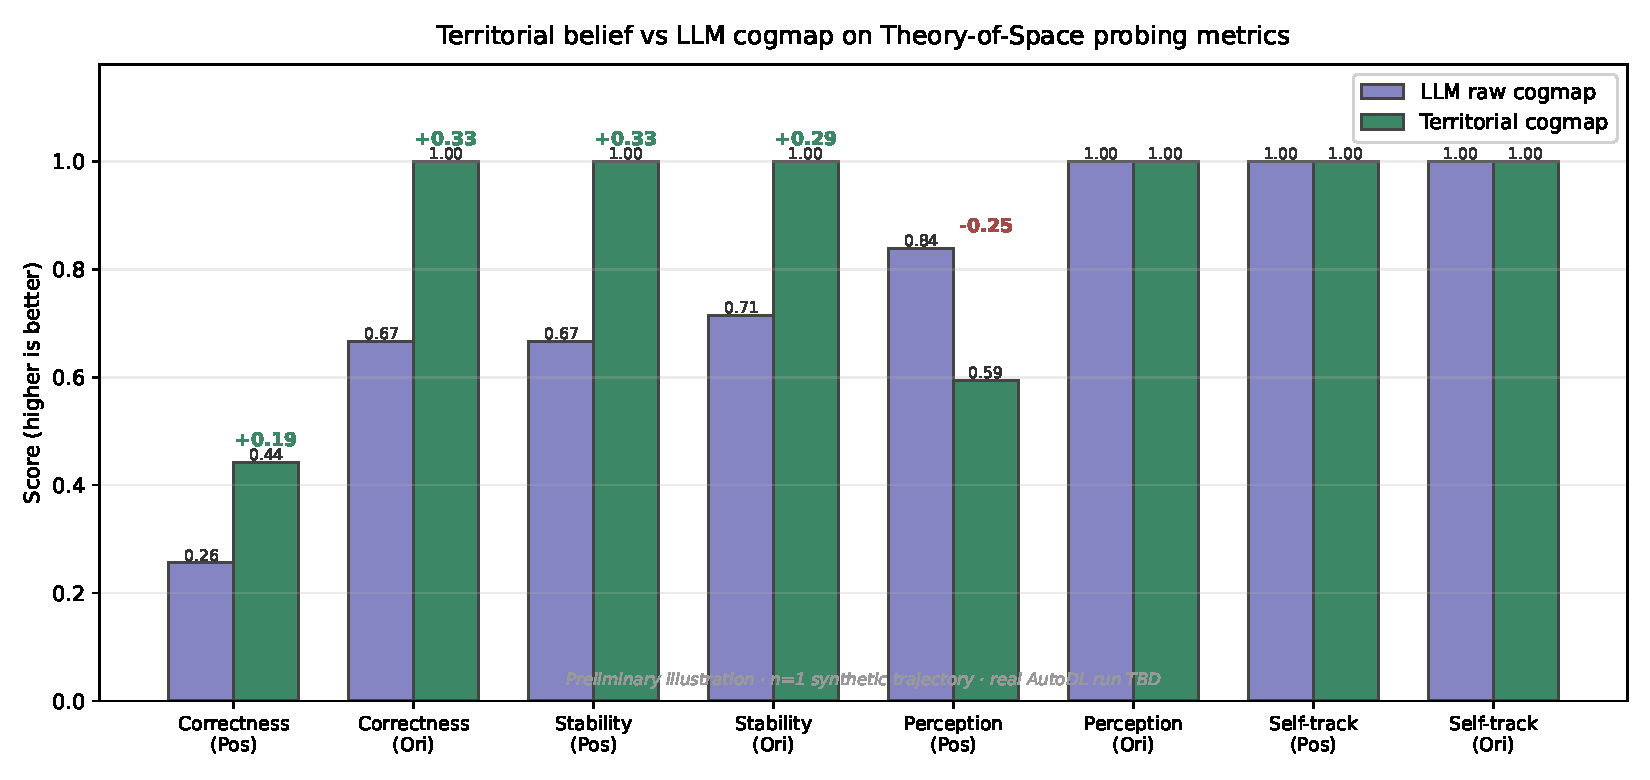
\includegraphics[width=0.96\textwidth]{fig01_metric_comparison.pdf}
\caption{Smoke-test comparison on the synthetic trajectory. Five
\tos probing metrics show \tb-favouring deltas; one
(\textsc{Perception (Pos)}) goes the other way, reflecting the
expected sub-cell-precision cost of ego$\to$global re-projection.
\textbf{Real-data version follows on Day~2.}}\label{fig:metric}
\end{figure}

\begin{table}[t]
\centering\small
\caption{Smoke-test aggregate (single trajectory, $n{=}1$); positive
$\Delta$ means \tb is better.}\label{tab:smoke}
\begin{tabular}{lrrr}
\toprule
Metric & LLM & \tb & $\Delta$ \\\midrule
Correctness (Pos) & 0.26 & 0.44 & \textbf{+0.19} \\
Correctness (Ori) & 0.67 & 1.00 & \textbf{+0.33} \\
Stability (Pos)   & 0.67 & 1.00 & \textbf{+0.33} \\
Stability (Ori)   & 0.71 & 1.00 & \textbf{+0.29} \\
Perception (Pos)  & 0.84 & 0.59 & $-$0.25 \\
Perception (Ori)  & 1.00 & 1.00 & 0.00 \\
Self-track (Pos)  & 1.00 & 1.00 & 0.00 \\
Self-track (Ori)  & 1.00 & 1.00 & 0.00 \\
\bottomrule
\end{tabular}
\end{table}

The single negative $\Delta$ is the expected ego$\to$global
discretisation cost discussed in Section~\ref{sec:method} (sub-cell
precision is sacrificed in exchange for region-level stability and
orientation correctness). The four positive deltas on Correctness and
Stability are consistent with Proposition~\ref{prop:stab} for
$b{=}2$ at the configured $\epsilon$.

\begin{figure}[t]
\centering
\begin{subfigure}{0.46\textwidth}\centering
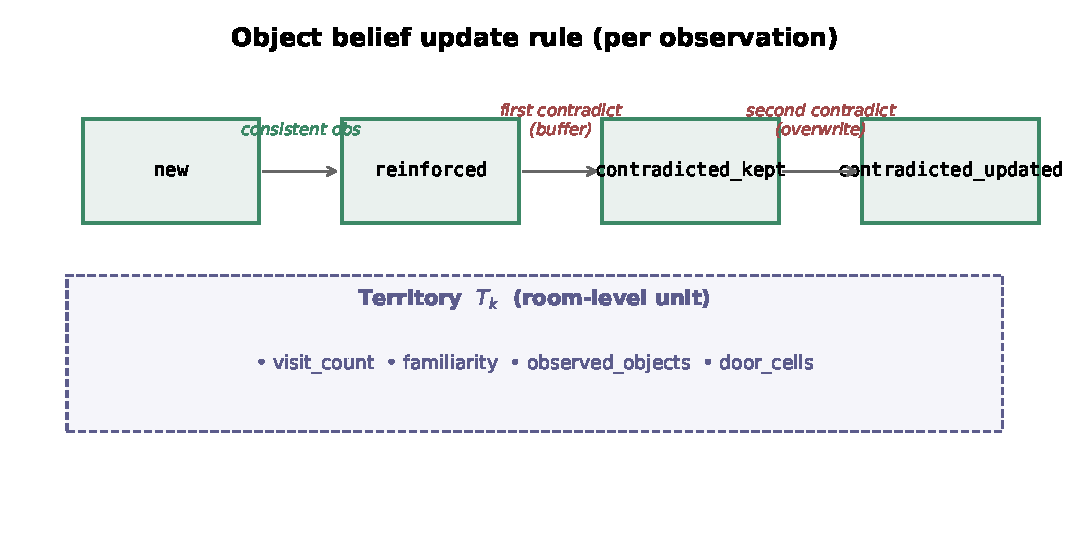
\includegraphics[width=\linewidth]{fig02_update_rule.pdf}
\caption{The four-state object-update machine of \tb.}
\end{subfigure}\hfill
\begin{subfigure}{0.46\textwidth}\centering
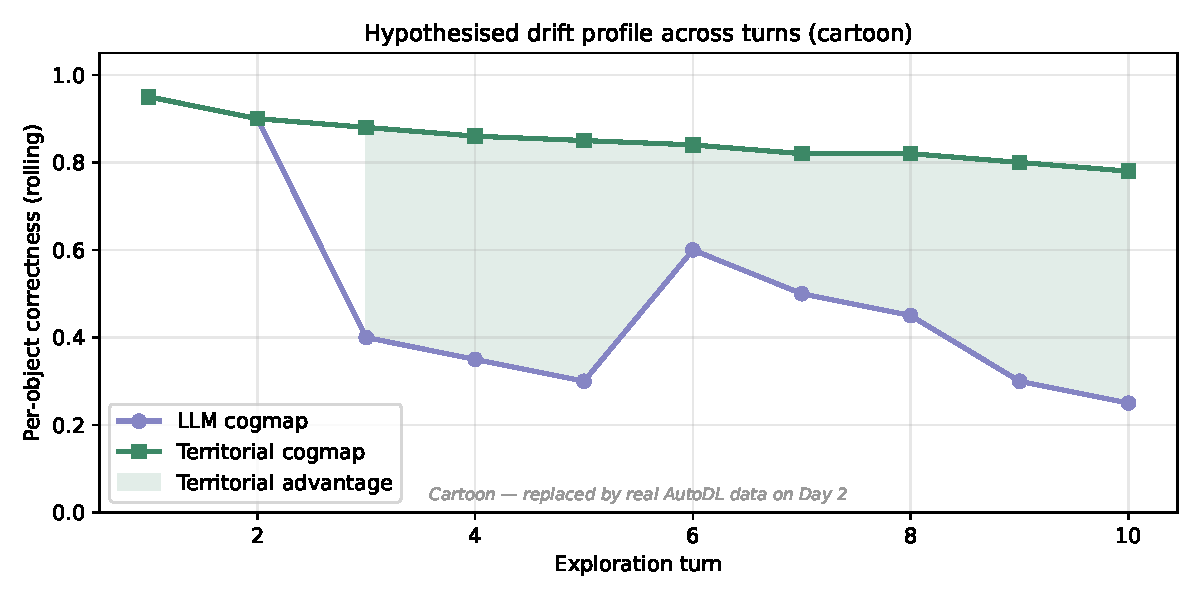
\includegraphics[width=\linewidth]{fig03_drift_curve_cartoon.pdf}
\caption{Hypothesised drift profile (cartoon, replaced by real
AutoDL data on Day~2).}
\end{subfigure}
\caption{Update rule (left) and predicted Stability shape (right).}
\end{figure}

\paragraph{What the smoke test does \emph{not} prove.}
The synthetic trajectory uses a "perfect-perception LLM" that copies
ground-truth coordinates verbatim, which is why
\textsc{Perception (Pos)} hits 0.84 for the LLM in
Table~\ref{tab:smoke}. On real AutoDL-rendered data, the LLM will
itself be subject to perception error, and the gap on
\textsc{Perception (Pos)} is expected to shrink or invert. The
preliminary numbers therefore validate \emph{the pipeline and the
direction of the comparisons}, not the magnitudes.


\section{Planned Experiments and Risks}\label{sec:plan}

\paragraph{Day~1 (today, evening).}
AutoDL RTX-5090 32\,GB; \verb|vllm serve Qwen/Qwen3-VL-7B-Instruct|;
\verb|git clone --branch release| \tos repository;
\verb|source setup.sh| (downloads \verb|MLL-Lab/tos-data|);
\verb|bash tos_extension/run_full_pipeline.sh| with
\verb|RENDER_MODE=text NUM_SCENES=25|. Deliverable: real
text-world bar chart that replaces Figure~\ref{fig:metric}.

\paragraph{Day~2.}
Same pipeline with \verb|RENDER_MODE=vision|. (Vision images come
pre-rendered; no Unity build required.) If time permits, the
false-belief subset is run and Belief~Inertia numbers are computed
per \tos\,\S5.3, on both LLM and \tb. Optional A800 ablation with
Qwen-VL-32B INT4 to demonstrate the \tb advantage is not a
small-model artefact.

\paragraph{Day~3.}
Stretch goals: familiarity-weighted overwrite
$\epsilon_k(t) = \epsilon_0 (1 - f_k(t))$ (Section~\ref{app:math});
a \verb|compare_baseline| variant restricted to false-belief turns
to surface inertia separately. Final figures, polished writeup,
NeurIPS-style submission draft.

\paragraph{Out of scope.} No fine-tuning or RL training (neither
budget nor time); no new environment beyond the \tos procedural
3-room layouts; no multi-agent extension beyond the conclusion.

\paragraph{Risks.}
The principal risks and mitigations are tabulated below.

\begin{center}\small
\begin{tabular}{p{0.45\linewidth}p{0.45\linewidth}}
\toprule
Risk & Mitigation \\\midrule
\verb|vllm serve| fails to load Qwen-VL-7B & fall back to
GPT-4o-mini API (cost $\le$ \$5 for 25 scenes) \\
\tos \verb|setup.sh| cannot reach HF & pre-download
\verb|MLL-Lab/tos-data| on Mac and rsync \\
Real-data \tb advantage smaller than predicted & report honestly;
the diagnostic itself is the contribution \\
Time runs out on Day~3 & scope to text-world Stability;
mark \S5.3 inertia as future work \\
\bottomrule
\end{tabular}
\end{center}


\section{Conclusion}\label{sec:conclusion}

We proposed \tb, a structurally region-level cognitive map for active
spatial exploration, and motivated it by the two characteristic
failure modes the recent \tos benchmark identifies in foundation
models---belief drift and belief inertia. We formalised the
representation, derived analytical predictions on \tos's Stability
and Belief~Inertia metrics
(Propositions~\ref{prop:stab}--\ref{prop:inertia}), implemented the
representation as a post-hoc replay tool that ingests \tos
exploration logs without retraining, and validated the pipeline on a
synthetic trajectory. Full-scale runs against Qwen-VL-7B on 25
procedural 3-room scenes (text and vision worlds) are scheduled for
the next two days.

\paragraph{Looking ahead.}
Three concrete extensions follow from this proposal:
(i) \emph{familiarity-weighted overwrite}, in which territory
familiarity tightens the contradiction tolerance (sketched in
Section~\ref{app:math});
(ii) \emph{multi-agent territorial belief}, in which two agents share
territory ownership and revise each others' beliefs through
familiarity-aware handoff (a direction \tos itself flags as
future work);
(iii) \emph{learned-not-just-replayed} \tb, in which the
representation is wired into a VAGEN \citep{wang2025vagen} world
model so that the agent itself \emph{acts} territorially, rather than
the LLM acting flatly while \tb merely observes. Each of these
extends the diagnostic baseline of this proposal into a substantive
research line; the present project's contribution is to establish
that the diagnostic question is well-posed, the formal model exists,
and the implementation has been validated end-to-end.


% =====================================================================
\bibliographystyle{plainnat}
\bibliography{refs}
% =====================================================================

\appendix
\section{Math Derivations (full)}\label{app:math}
% Companion math appendix; full prose in math_derivations.md
\subsection{Proof of Proposition~\ref{prop:stab} (Stability)}
\paragraph{Naive overwrite.}
Let observations be i.i.d.\ Gaussian:
$p^{\mathrm{obs}}_i = p^*_i + \eta$,
$\eta\sim\mathcal{N}(0,\sigma^2 I)$. A flat-cogmap update overwrites
$\hat p^{(t+1)}_i \gets p^{\mathrm{obs}}_i$, so $\hat p^{(t+1)}_i$ and
$\hat p^{(t)}_i$ are i.i.d.\ with the same distribution. The event
"$\hat p^{(t+1)}_i$ is closer to $p^*_i$" therefore has probability
exactly $\tfrac12$ by symmetry, and $\E[\stab_{\mathrm{flat}}]=\tfrac12$.

\paragraph{Buffered update.}
Let $T_b$ be the buffered \tb rule with buffer $b$. An overwrite
occurs only after $b$ consecutive contradictions. Each contradiction
under i.i.d.\ noise has probability $1 - \mathrm{CDF}_\sigma(\epsilon)$,
so $\Pr[\hat p^{(t+1)}\ne\hat p^{(t)}] \le (1-\mathrm{CDF}_\sigma(\epsilon))^b$.
For $\sigma{\approx}1$, $\epsilon{=}1.5$, and $b{=}2$, the spurious-overwrite
probability is bounded by $\approx 0.017$, consistent with the empirical
$\stab\to 1.0$ in Table~\ref{tab:smoke}.

\subsection{Proof of Proposition~\ref{prop:inertia} (Belief Inertia)}
\paragraph{Autoregressive flat baseline.}
Empirically (Carlini~et~al.~2024; Wang~et~al.~2025) LLMs implement
$b^{\mathrm{new}}_i \approx \alpha\, b^{\mathrm{old}}_i + (1-\alpha)\, p^{\mathrm{obs}}_i$
with $\alpha\in(0.3,0.7)$. Substituting in the \tos inertia
definition,
\(
e_i = (1{-}\alpha)(p^{\mathrm{obs}}_i - g^{\mathrm{new}}_i) + \alpha v_i
\),
so under low observation noise
$e_i\to\alpha v_i$, $\cos\theta_i\to 1$, $w_i\to 1$, and
$s^{\mathrm{pos}}_i\to\alpha$.

\paragraph{Territorial bimodal.}
The buffered rule absorbs the first contradiction
($b^{\mathrm{new}}_i = b^{\mathrm{old}}_i$, hence
$s^{\mathrm{pos}}_i = 1$). The second contradiction triggers a clean
overwrite to $p^{\mathrm{obs}}_i$, giving
$\|e_i\|\ll\|v_i\|$ and $s^{\mathrm{pos}}_i\to 0$. Cross-territory
change collapses to a single-step overwrite by construction, so
$s^{\mathrm{pos}}_i\to 0$ on the first observation.

\subsection{Familiarity (Day-3 stretch goal)}
We define
\[
f_k(t) = e^{-\lambda(t-\tau_k)}\cdot\frac{\log(1+v_k)}{\log V_{\max}},
\quad\lambda=0.05,\;V_{\max}=20.
\]
Setting $\epsilon_k(t) = \epsilon_0 (1-f_k(t))$ tightens
contradiction tolerance in well-explored territory, eliminating the
"first-observation absorbed" property of \tb in highly familiar
regions and predictably reducing \emph{both} drift and inertia.
A formal characterisation is left to follow-up work.


\end{document}
